\section{Theory and Procedure}

% a) Aim of the Experiment or Abstract (2 marks)
% b) Apparatus/Instruments ( 2 marks)
% c) Procedure and circuit diagram along with theory (6 marks)
% d)Observation table with graph (10 marks).
% e) Discussion on Analysis of deviation from the expected value (This should cover the reason why we do not get ideal gain or ideal characteristics as expected from formula) (4 marks)
% f) Precaution and Conclusion (2 mark)
% g) Applications with associated circuit if any ( 4 marks)  (Additional Section)

% \end{enumerate}

\subsection*{Introduction}

One of the most versatile and widely used electronic devices in linear applications is the operational amplifier, most often referred to as the op-amp. Op amps are popular because they are low in cost and easy to use. Op amps have five basic terminals: two for supply power, two for input signals, and one for output. Inverting input marked with a negative sign, and the other a non-inverting input marked with a positive plus sign.\\

The ideal op amp (Fig. \ref{fig:0}) has infinite gain which is frequency independent. The input terminals draw no current and exhibit infinite input resistance. Output impedance is 0 $\Omega$, so that maximum voltage can be drawn by the load.
The amplified output signal of an Operational Amplifier is the difference between the two signals being applied to the two inputs. Since an op-amp is an active device,  power supply is provided to the op-amp using a bipolar supply and has typical values of $\pm$ 15 V.\\

\begin{figure}[H]
    \centering
    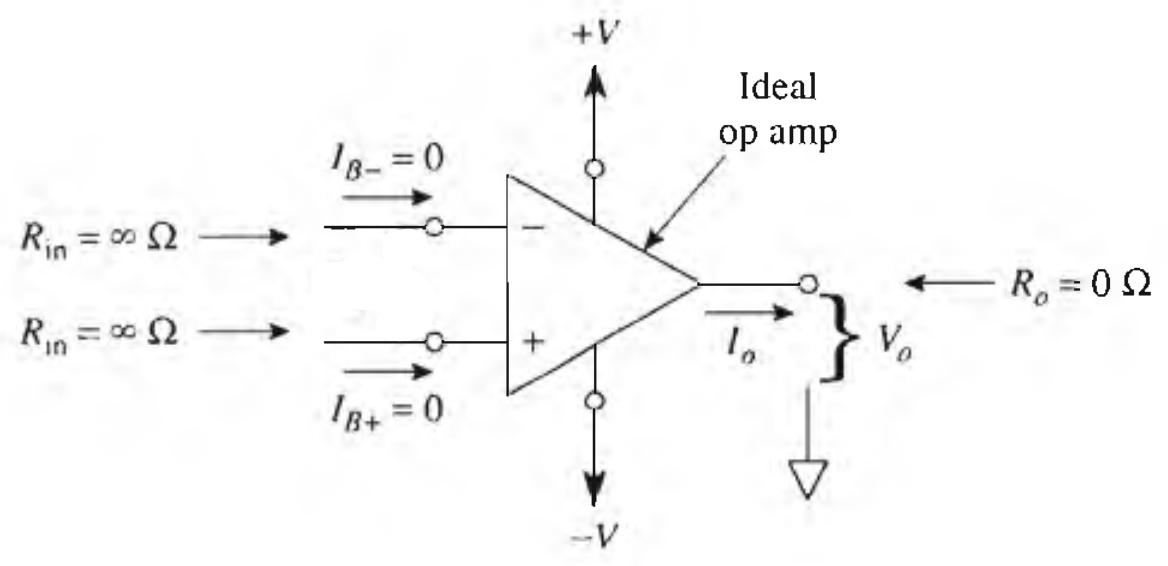
\includegraphics[width=0.90\columnwidth]{images/ideal.png}
    \caption{Schematic of an ideal op-amp\\}
    \label{fig:0}
\end{figure}

The most commonly available and used of all operational amplifiers is the industry standard 741 type IC. 

\begin{figure}[H]
    \centering
    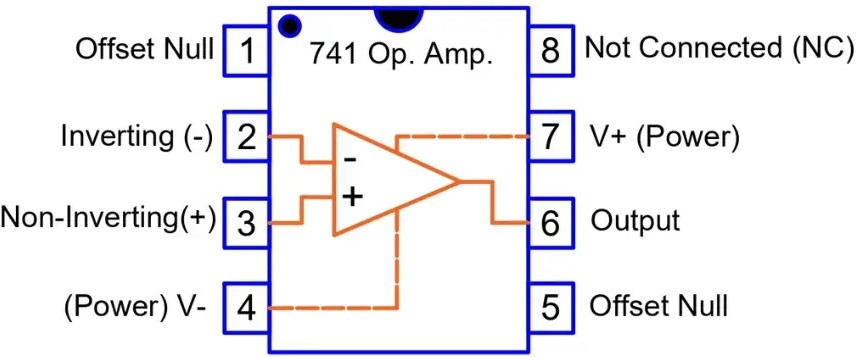
\includegraphics[width=0.95\columnwidth]{images/pinout.jpeg}
    \caption{IC 741 Pinout}
    \label{fig:1}
\end{figure}

The output voltage $V_\text{out}$ is determined by the open loop gain (without any possible feedback connections), is given by 

\begin{align}V_\text{out}=A_{OL}(V_1-V_2)\end{align} 

\textbf{Open loop gain} or DC gain of an ideal Operational Amplifier can be very high, (around $10^6$), making the amplifier hard to control as the smallest of input signals can cause the output to saturate and the input signal will lose its characterstics. Hence by losing some of this gain by connecting a suitable resistor across the amplifier from the output terminal back to the inverting input terminal, we can both reduce and control the overall gain of the amplifier. This then produces an effect called \textbf{Negative Feedback}, and thus produces a very stable Operational Amplifier system. The resulting gain is called its \textbf{closed loop gain}.



To separate the real input signal from the negative feedback voltage at the inverting terminal, we use the input resistor $R_\text{in}$. As we are not using the positive non-inverting input this is connected to a common ground.
The effect of this closed loop feedback circuit results in the voltage at the inverting input equal to that at the non-inverting input producing a \textit{Virtual Earth} summing point because it will be at the same potential as the grounded reference input. 

% ======================================================================================
\subsection{Inverting Amplifier Circuit}

\begin{figure}[H]
    \centering
    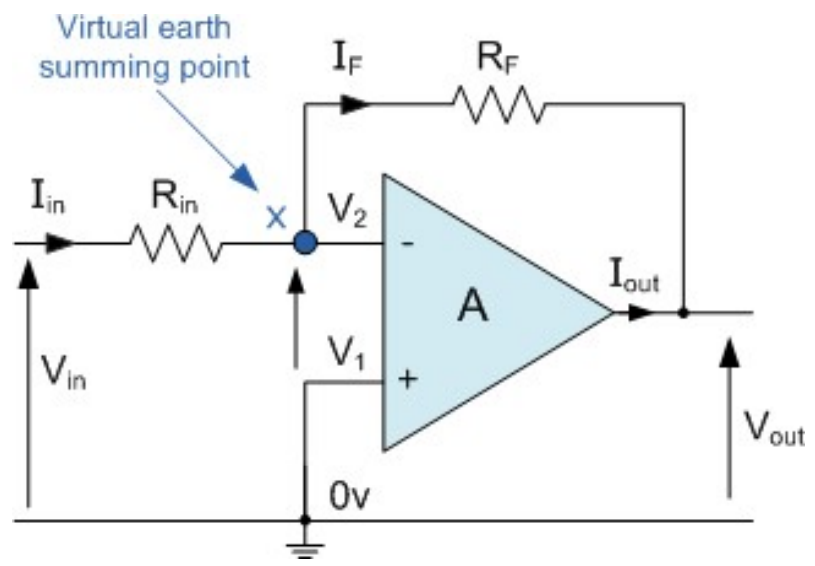
\includegraphics[width=0.7\columnwidth]{images/inv1.png}
    \caption{Inverting Amplifier Circuit}
    \label{inv1}
\end{figure}

In inverting amplifier circuit the operational amplifier is connected with feedback to produce a closed loop operation. Here, no current flows into the input terminal. Also, $V_1$ equals $V_2$ since the junction of the input and feedback signal is at the same potential as the positive (+) input which is at zero volts or ground and thus the junction is a \textit{Virtual Earth}. Thus input resistance of the amplifier is equal to the value of the input resistor, $R_\text{in}$.

\begin{figure}[H]
    \centering
    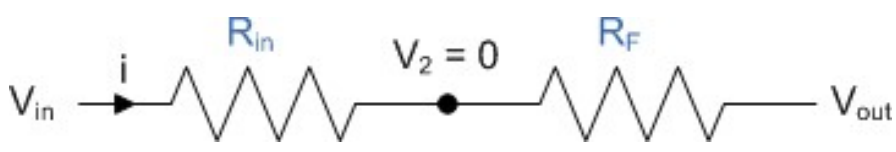
\includegraphics[width=0.8\columnwidth]{images/inv2.png}
    \caption{Inverting Amplifier Equivalent Circuit}
    \label{inv2}
\end{figure}

We can calculate the gain of this configuration by using the equivalent circuit (Fig. \ref{inv2}) the circuit to get,

\begin{align}
    i = \frac{V_\text{in}}{R_\text{in}} &= -\frac{V_\text{o}}{R_f} \nonumber \\
    \implies \text{Gain, } A &= \frac{V_\text{o}}{V_\text{in}} = -\frac{R_f}{R_\text{in}} \label{inv gain}
\end{align}

The negative sign indicates a phase difference of $\pi$ of the output signal with respect to the input signal.

% \subsubsection*{Experimental Procedure to find the Gain of the Inverting Amplifier}

% \begin{enumerate}
%     \item Configure the circuit as shown in the circuit diagram (Fig. \ref{inv3}). Connect the pins 7 and 4 of the IC to the $\pm$15V output terminals of the DC power supply. Connect the 0V terminal to ground. Choose $R_\text{in}$ = 1 k$\Omega$ and $R_f$ = 10 k$\Omega$ and calculate gain. Connect $R_3 = R_\text{in} \parallel R_f \approx R_\text{in}$ to minimize offset due to input bias current. 
%     \item Connect one of the output terminals of the D.C. power supply (0-30V) at the inverting input pin (2).
%     \item Switch on the power supply and apply different voltages in the
%     range 0-1.5V at the inverting terminal. Measure this input and the corresponding output voltages with the multimeter and calculate gain. Note the sign of the output voltage.
%     \item Replace $R_f$ by 50 k$\Omega$ and repeat the procedure and notice the changes.
    
% \end{enumerate}

\begin{figure}[H]
    \centering
    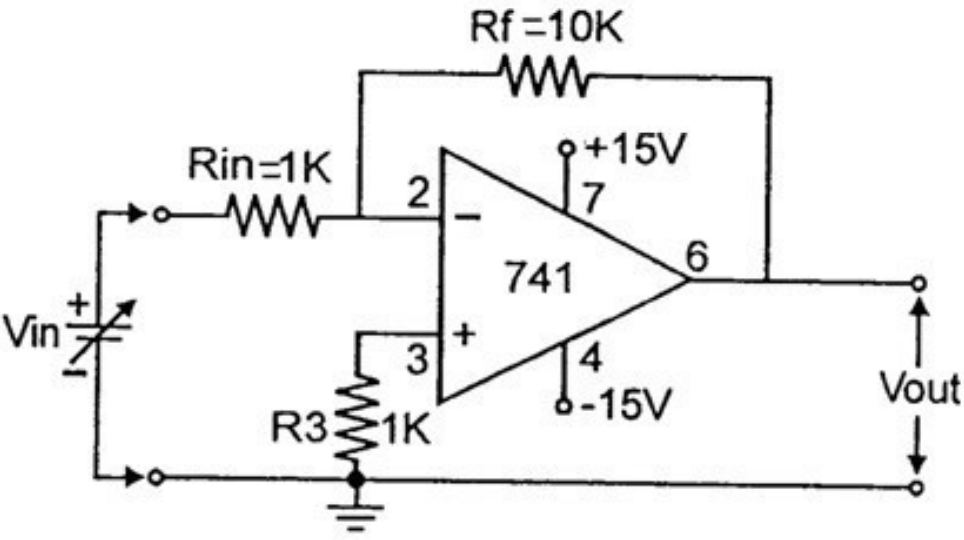
\includegraphics[width=0.8\columnwidth]{images/inv3.png}
    \caption{Experimental Circuit Diagram for Inverting Amplifier}
    \label{inv3}
\end{figure}

One of its undesirable feature is the low input impedance, particularly for amplifiers with large closed-loop voltage gain, where $R_1$ tends to be rather small. This is remedied in case of a non-inverting amplifier. 

% ======================================================================================

\subsection{Non-Inverting Amplifier Circuit}

\begin{figure}[H]
    \centering
    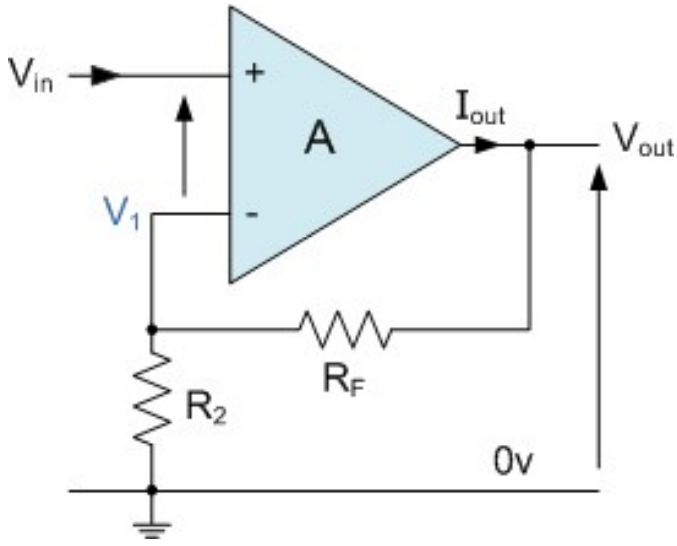
\includegraphics[width=0.6\columnwidth]{images/noninv1.png}
    \caption{Non-Inverting Amplifier Circuit}
    \label{noninv1}
\end{figure}

In this configuration, the input voltage signal, ($V_\text{in}$) is applied directly to the Non-inverting (+) input terminal. By applying a small part of the output voltage signal back to the inverting (-) input terminal via a $R_f - R_2$ voltage divider network, producing negative feedback, we can achieve very good stability, $R_\text{in} \rightarrow \infty$ (as no current flows into the positive input terminal) and a low output impedance, $r_\text{out}$.

\begin{figure}[H]
    \centering
    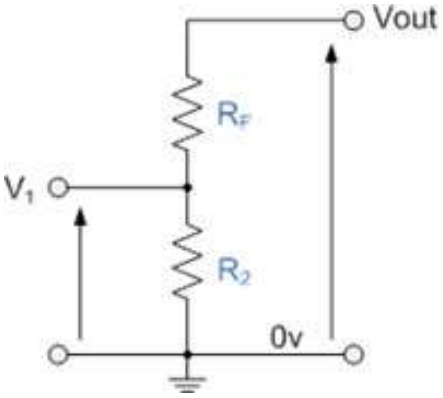
\includegraphics[width=0.45\columnwidth]{images/noninv2.png}
    \caption{Non-Inverting Amplifier Equivalent Voltage Divider Circuit}
    \label{noninv2}
\end{figure}

Since $V_1 = V_\text{in}$, the junction is a \text{Virtual Earth} summing point. $R_f$ and $R_2$ form a voltage divider network across the amplifier. Using the equivalent circuit (\ref{noninv2}), we get,

\begin{align}
    V_\text{out} &= V_\text{in} \left(1+\frac{R_f}{R_2}\right) \nonumber\\
    A &= \frac{V_\text{o}}{V_\text{in}} = 1 + \frac{R_f}{R_2}
\end{align}

Here, the gain is positive or the output signal is in-phase with the input signal.

% \subsubsection*{Experimental Procedure to find the Gain of the Non-Inverting Amplifier}

% \begin{enumerate}
%     \item Configure the circuit as shown in the circuit diagram (Fig. \ref{noninv3}) with $R_\text{in}$ = 1 \kohm\,and $R_f$ = 10 \kohm. Calculate gain using the measured value of resistance.
%     \item Connect one of the output terminals of the D.C. power supply (0-30V) at the non-inverting input pin (3).
%     \item Repeat steps 3 onwards as described in the case of inverting amplifier.
% \end{enumerate}

\begin{figure}[H]
    \centering
    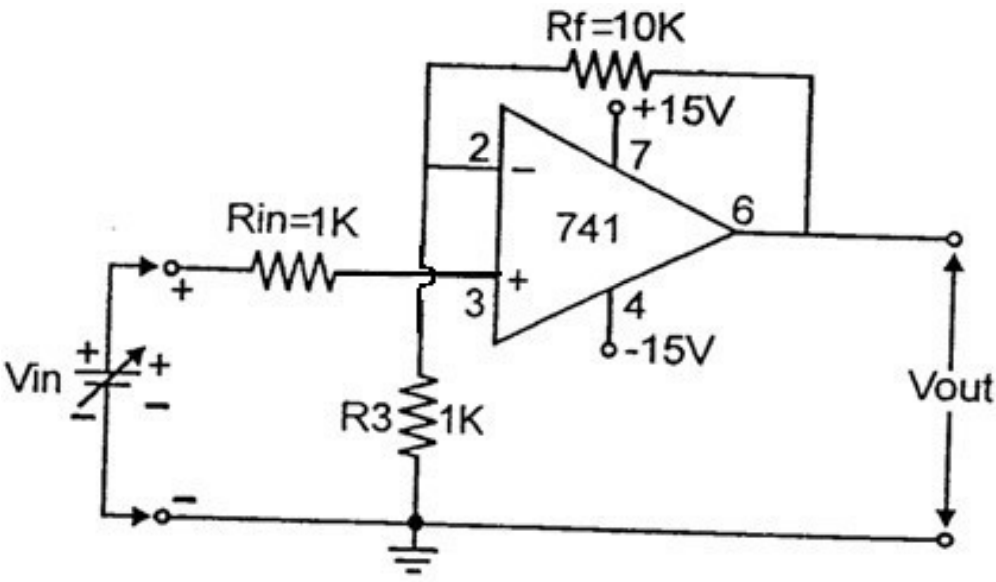
\includegraphics[width=0.8\columnwidth]{images/noninv3.png}
    \caption{Experimental Circuit Diagram for Non-Inverting Amplifier}
    \label{noninv3}
\end{figure}

% ======================================================================================

\subsection{OPAMP as a Summing Amplifier}

\begin{figure}[H]
    \centering
    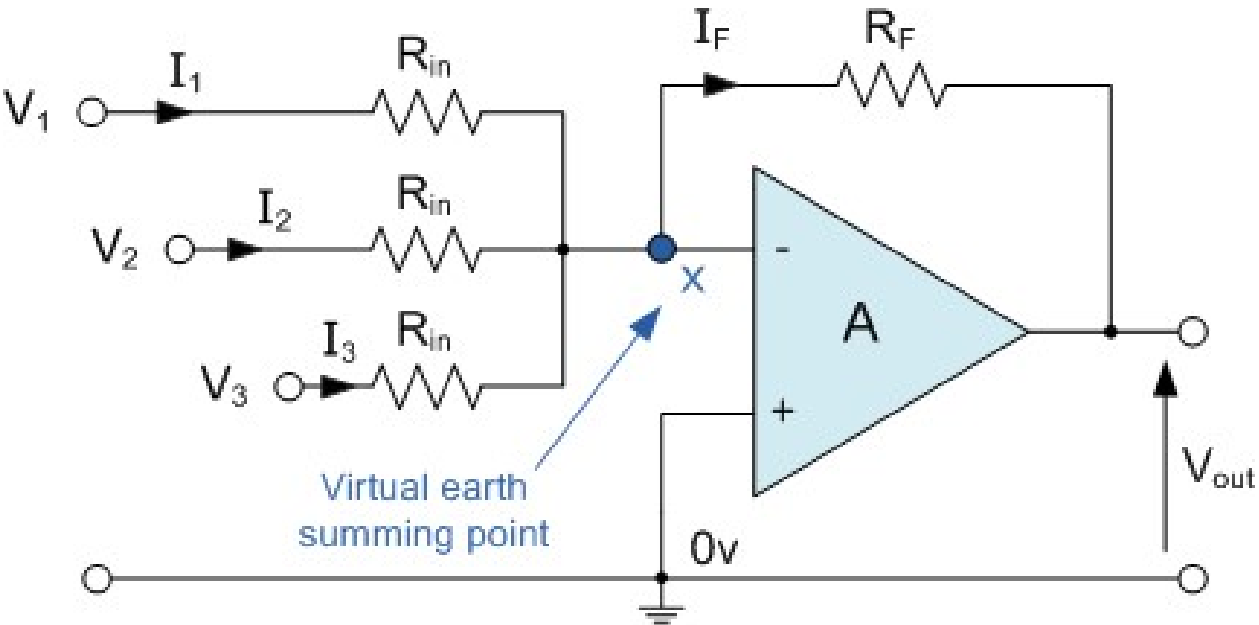
\includegraphics[width=0.8\columnwidth]{images/sum1.png}
    \caption{Summing Amplifier Circuit}
    \label{sum1}
\end{figure}

If we add another input resistor equal in value to the original input resistor, $R_\text{in}$ in Fig. \ref{inv1} we end up with another operational amplifier circuit called a Summing Amplifier or a \textit{Voltage Adder} circuit (Fig. \ref{sum1}). The output voltage, ($V_\text{out}$) thus becomes proportional to the sum of the input voltages, $V_1, V_2, V_3, \dots$. Using the original equation for the inverting amplifier (Eq. \ref{inv gain}),

\begin{align}
    I_f &= I_1 + I_2 + I_3 \nonumber \\
    V_\text{out} &= -I_f R_f \nonumber \\
    &= -R_f \left(\frac{V_1}{R_1} + \frac{V_2}{R_2} + \frac{V_3}{R_3}\right) \nonumber \\
    &= -\frac{R_f}{R_\text{in}} (V_1 + V_2 + V_3) \nonumber \\
    &= A_v (V_1 + V_2 + V_3)
\end{align}

if $R_1 = R_2 = R_3 = R_\text{in}$, and thus $A_v=-R_f/R_\text{in}$.

Hence this enables us to effectively add together several individual input signals. Additionally, if the input resistors are of different values a \textit{scaling summing amplifier} is produced which gives a weighted sum of the input signals.

% \subsubsection*{Experimental Procedure to  study OPAMP as Summing Amplifier}

% \begin{enumerate}
%     \item Assemble the circuit as shown in circuit diagram (Fig. \ref{sum2}) and choose $R_1, R_2, R_f=$  10 \kohm each. Use 0-$\pm$15V terminal output to provide supply to the IC.
%     \item Using 0-30V and 5V terminals of the power supply, apply two inputs at the inverting terminal. Measure each input with multimeter.
%     \item Measure the output with multimeter for differnet input combinations and compare the output with the sum of the two inputs.
% \end{enumerate}

\begin{figure}[H]
    \centering
    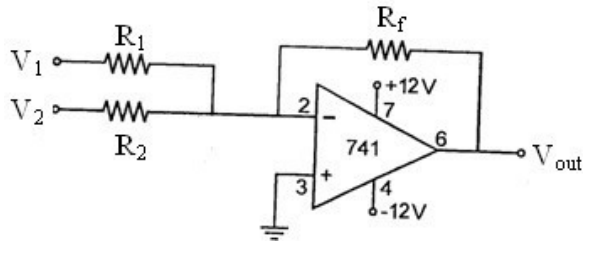
\includegraphics[width=0.8\columnwidth]{images/sum2.png}
    \caption{Experimental Circuit Diagram for Summing Amplifier}
    \label{sum2}
\end{figure}

% ======================================================================================
\subsection{OPAMP as a Difference Amplifier}

\begin{figure}[H]
    \centering
    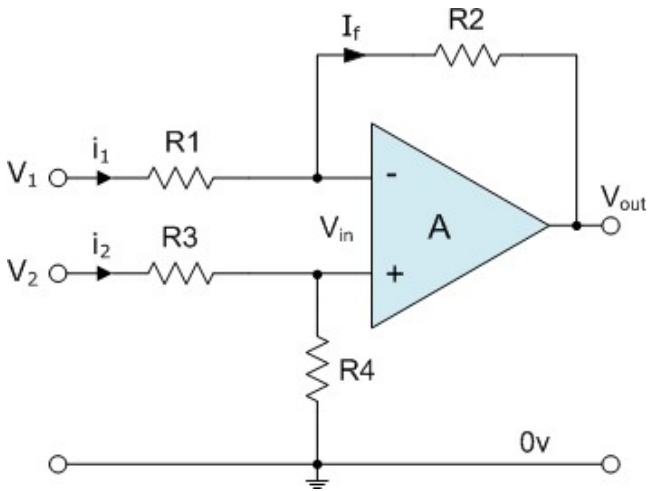
\includegraphics[width=0.8\columnwidth]{images/diff1.png}
    \caption{Difference Amplifier Circuit}
    \label{diff1}
\end{figure}

If we connect input signals to both inverting and non-inverting terminals simultaneously, the resultant output voltage will be proportional to the difference between the two input signals, $V_1$ and $V_2$. This type of circuit can be used as a subtractor.

\begin{align}
    V_o &= -\frac{R_1}{R_2}V_1 + \left(1+\frac{R_1}{R_2}\right)\left(\frac{R_4}{R_3+R_4}\right)V_2 \nonumber \\
    &= \frac{R_2}{R_1}(V_2-V_1)
\end{align}

if $R_1 = R_2$ and $ R_3 = R_4$.

% Hence this enables us to effectively add together several individual input signals. Additionally, if the input resistors are of different values a \textit{scaling summing amplifier} is produced which gives a weighted sum of the input signals.

% \subsubsection*{Experimental Procedure to  study OPAMP as Difference Amplifier}

% \begin{enumerate}
%     \item Assemble the circuit as shown in circuit diagram (Fig. \ref{diff2}) and choose $R_1, R_2, R_f=$  10\,\kohm each. Use 0-$\pm$15V terminal output to provide supply to the IC.
%     \item Using 0-30V and 5V terminals of the power supply, apply two inputs at the inverting terminal. Measure each input with multimeter. 
%     \item Measure the output with multimeter for differnet input combinations and compare the output with the difference of the two inputs.
% \end{enumerate}

\begin{figure}[H]
    \centering
    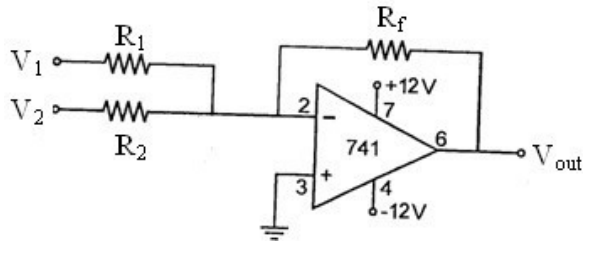
\includegraphics[width=0.8\columnwidth]{images/sum2.png}
    \caption{Experimental Circuit Diagram for Difference Amplifier}
    \label{diff2}
\end{figure}
% ======================================================================================
\subsection{OPAMP as a Comparator}

\begin{figure}[H]
    \centering
    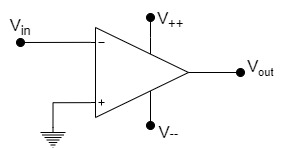
\includegraphics[width=0.8\columnwidth]{images/comparator.jpg}
    \caption{Circuit Diagram for a Comparator Circuit}
    \label{comp1}
\end{figure}

Without negative feedback, the op-amp goes into positive or negative saturation according to the difference of the input voltages, which can be used to design switching or non-linear circuits.

From the circuit diagram (Fig. \ref{comp1}) we can see that, 
% if $V_\text{in} > 0, V_o \approx V_{++}$ and $V_\text{in} < 0, V_o \approx V_{--}$. 
\begin{align}
    V_\text{out} \approx \begin{cases}
        V_{++} \text{ if } V_+ > 0\\
        V_{--} \text{ if } V_+ < 0\\
    \end{cases}
\end{align}
Hence, the circuit can be used as a comparator.

If we modify the circuit a bit by connecting the non-inverting terminal to a any voltage source, $V_{th}$ (Fig. \ref{comp2}), the circuit now switches when $V_\text{in}$ crosses a the threshold value $V_\text{th}$.

\begin{figure}[H]
    \centering
    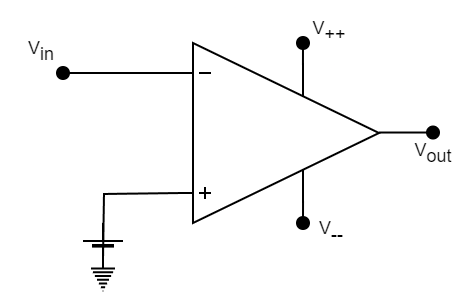
\includegraphics[width=0.8\columnwidth]{images/comp2.png}
    \caption{Circuit Diagram for a Comparator Circuit with a certain threshold voltage}
    \label{comp2}
\end{figure}

This simple comparator circuit is \textit{not ideal} for practical use, i.e. if the input is noisy, the output may make several transitions as the input passes through the threshold point (Fig. \ref{comp3}). Also, for very slowly varying input, the output transitions can be rather slow. These can be remedied by using the \textit{Schmitt trigger}.

\begin{figure}[H]
    \centering
    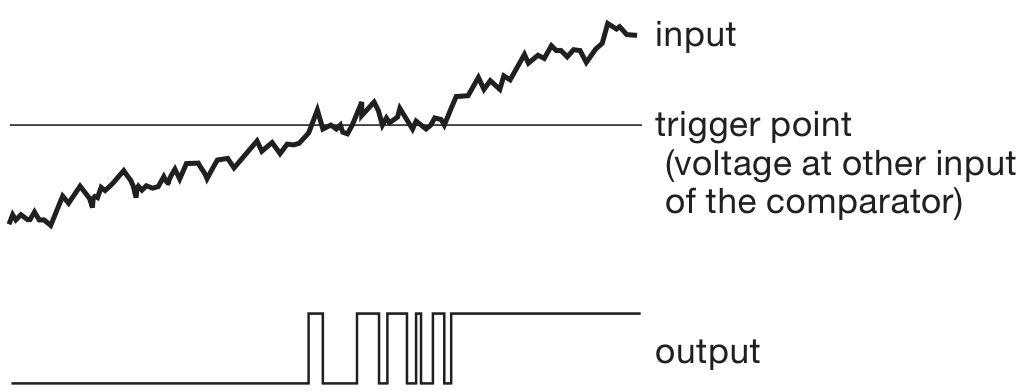
\includegraphics[width=0.85\columnwidth]{images/comp3.png}
    \caption{Comparator output for the corresponding input signal}
    \label{comp3}
\end{figure}

% \subsubsection*{Experimental Procedure to study the OPAMP as a Voltage Comparator}

% \begin{enumerate}
%     \item Construct the comparator circuit on the breadboard as shown in the circuit diagram (Fig. \ref{comp1}).
%     \item Use terminal C of the DC. power supply to providepower supply to IC.
%     \item Connect terminal A of the d.c. power supply (0-30V) at the input. Use terminal B (5V) to provide threshold voltage $V_\text{th}$ for circuit shown Fig. \ref{comp2}.
%     \item Vary the input from a negative value to a positive value through 0 and measure and tabulate $V_\text{in}$ and $V_o$. 
%     \item Plot $V_\text{in}$ vs. $V_o$ and estimate $V_\text{th}$.

% \end{enumerate}

% ======================================================================================
\subsection{OPAMP as Schmitt trigger}

The Schmitt Trigger is a modification on the comparator circuit with positive feedback. This causes the circuit to to have two threshold points --- when the output is high, it makes the switching level higher than it is when the output is low. This causes the circuit to have hysteresis or toggle action.
Thus, noisy inputs are less likely to output multiple triggering.

Let $V_+$ and $V_-$ be the voltages at the non-inverting and inverting terminals respectively.
Since $V_\text{out}$ changes its state whenever $V_+$ crosses 0V, we need to find what value of $V_\text{in}$ results in $V_+ = 0$. The two values of $V_\text{in}$ for which the output switches are called the \textit{trip points}. $V_+ = 0$ acts as a voltage divider formed by $R_1$ and $R_2$ between $V_\text{in}$ and $V_\text{out}$. Thus the trip points of a non-inverting Schmitt trigger are: 

\begin{align}
    V_\text{in} = \begin{cases}
        -(R_1/R_2)V_\text{out} \text{ (Lower trip point, LTP)}\\
        +(R_1/R_2)V_\text{out} \text{ (Upper trip point, UTP)}\\
    \end{cases}
\end{align}

Choosing suitable ratios of $R_1$ to $R_2$, enough hysteresis can be created in order to prevent unwanted noise triggers. 

\begin{figure}[H]
    \centering
    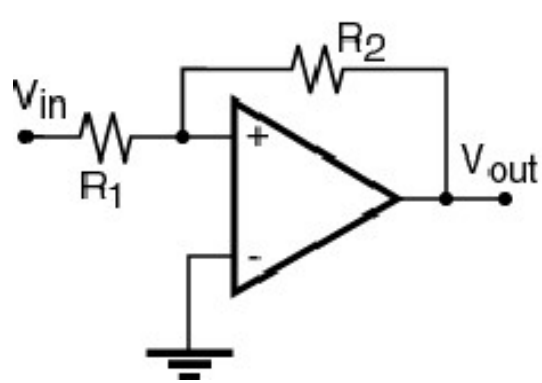
\includegraphics[width=0.5\columnwidth]{images/schmitt.png}
    \caption{Schmitt trigger circuit diagram}
    \label{schmitt}
\end{figure}

% ======================================================================================
\section{Apparatus}

\begin{enumerate}
    \item OPAMP 741 Chip
    \item Resistors
    \item DC Power Supply
    \item Breadboard
    \item Connecting Wires
    \item Multimeters
\end{enumerate}